\section{Convergencia en Ley}
    

\hspace{3.5mm}Partiremos este capítulo enunciando uno de los teoremas más importante de la teoría de probabilidades, el teorema del límite central.

\begin{teorema}[Teorema Central del Límite.] Dadas $(X_n)_{n\in\N}$ variables aleatorias $i.i.d.$, con \newline$\mu = \E(X_1)$ y $\sigma^2 = Var(X_1)$, finitas. Para el promedio $n-$esimo:
\begin{equation}
    \overline{X}_n = \frac{1}{n}\sum_{i=1}^{n}X_i
\end{equation}
Se define la variable aleatoria $Z_n$ como:
\begin{equation}
    Z_n = \frac{\overline{X}_n - \mu}{\sigma / \sqrt{n}}
\end{equation}
Entonces $Z_n$ converge \textbf{\textit{"EN LEY"}} a una variable normal estándar $\mathcal{N}(0,1)$ a medida que $n$ tiende a infinito.
\end{teorema}

Los resultados y usos que se desprenden de este teorema son bastante variados; desde el cálculo de probabilidades para una muestra aleatoria simple, estimación de parámetros, hasta nos permite el uso de test de hipótesis para distribuciones normales en ocasiones en que desconocemos por completo la distribución de los datos.\footnote{Todos estos usos están restringidos bajo aproximaciones.}\\

Y no es que sea raro encontrar este tipo de usos, puesto que el teorema no nos pide absolutamente nada con respecto al tipo de  distribución de las variables aleatorias, dando la posibilidad de que éstas sean continuas, discretas o cualesquiera que se nos pudiesen ocurrir en diversos espacios de trabajo. Sin embargo el resultado es el mismo, convergencia a una distribución absolutamente continua.\\ 

Si $Z_n$ puede tomar varias formas dada la colección de variables $(X_n)_{n\in\N}$, ¿por qué converge a una distribución continua? Para responder esta pregunta introduciremos las nociones de \textit{convergencia débil de medida de probabilidad}.

\subsection{Convergencia débil sobre espacios métricos}

\hspace{3.5mm}Para el conjunto de medidas de probabilidad sobre el espacio métrico $E$, es decir; $\mathcal{P}(E)$, definiremos la siguiente operación.
\begin{definicion}
Para toda $\mu \in \mathcal{P}(E)$ y para toda $f: E\rightarrow \R$ función medible:
\begin{equation}
    \langle \mu , f\rangle = \int_{E} f d\mu
\end{equation}
Además diremos que una sucesión $(\mu_n)_{n\in\N}$ de elementos de $\mathcal{P}(E)$ converge \textbf{DÉBILMENTE} a $\mu\in \mathcal{P}(E)$ si:
\[\langle \mu_n ,f\rangle\, \xrightarrow{n\rightarrow\infty}\, \langle \mu,f\rangle \hspace{0.5cm}\forall\,f\in C_b(E)\]
En tal caso anotamos: $\mu_n \Rightarrow \mu$.
\end{definicion}
\textbf{Ejemplo 1:} Tomemos el espacio métrico $E=\R$ con su métrica usual $d(x,y) = |x-y|$, y sea la sucesión de medidas de probabilidad $\mu_n = \delta_{\frac{1}{n}}$, donde $\delta_a$ representa la "Delta de Dirac" en el punto $a$:
    \[\delta_a(x) = \begin{cases} 
            +\infty & \text{si }x=a   \\ 
            0 & \text{si }x\neq a \end{cases}\]
    
    Veremos que esta distribución converge débilmente a la distribución $\delta_0$.\\
    En efecto, sea $f \in C_b(\R)$, tenemos que:
    \[\langle \mu_n ,f\rangle = \int_\R f(x) \mu_n (dx) = \int_\R f(x) \delta_{\frac{1}{n}}(x) dx = f(1/n)\]
    Puesto que la función $f$ es continua en todo $\R$, entonces:
    \[f(1/n) \xrightarrow{n\rightarrow\infty}\,f(0) = \langle \mu,f\rangle \]
    Por lo tanto, $\mu_n \Rightarrow \mu$.
\\

Dado que el argumento utilizado en el ejemplo se sostuvo fuertemente de la continuidad de la función $f$, en general se tendrá que para cada sucesión de reales $(x_n)_n$ que converja a un punto $\Bar{x}$, se tendrá la convergencia de las medidas de Dirac: $\delta_{x_n}\Rightarrow \delta_{\Bar{x}}$. Se puede demostrar que esto es una doble implicancia, es decir; la convergencia debil de las medidas de Dicar implican la convergencia en $\R$ de la sucesión de los puntos.\\

Para traducir el \textit{Teorema Central del Límite} en conceptos de convergencia de medidas de probabilidad debemos asociar el concepto de \textit{variable aleatoria} en función de la medida de probabilidad asociada.\\

Recordemos que una \textbf{variable aleatoria} a valores en $E$ es una función $X:\Omega \rightarrow E$ medible, donde $(\Omega, \mathcal{F},\pb)$ es un espacio de probabilidad (este espacio se encuentra usualmente implícito en la mayoría de las definiciones y cálculos de probabilidades).\\ 
Su \textbf{LEY} o \textbf{DISTRIBUCIÓN}, denotada como $\mathcal{L}(X) \in \mathcal{P}(E)$, se define como:
\begin{equation}
   \mathcal{L}(X)(A) := \pb(X^{-1}(A))\hspace{0.5cm}\forall\,A\in\mathcal{B}(E) 
\end{equation}

\begin{definicion} Una sucesión $(X_n)_{n\in\N}$ de variables aleatorias en $E$ se dice que converge \textbf{EN LEY} o \textbf{EN DISTRIBUCIÓN} a una variable aleatoria $X$ si $(\mathcal{L}(X_n))_{n\in\N}$ converge débilmente a $\mathcal{L}(X)$, es decir:
\[\E[f(X_n)] \xrightarrow{n\rightarrow\infty}\,\E[f(X)]\hspace{0.5cm}\forall\,f\in\,C_b\]
En este caso anotamos: $X_n\,\xrightarrow{\mathcal{L}}\,X$ o $X_n\,\xrightarrow{d}\,X$.
\end{definicion}

Notamos que esta definición es idéntica a la anterior pero expresada en términos de la esperanza de la función $f$ en vez de la integral de la función bajo la medida de probabilidad.\\\newline
\textbf{Ejemplo 2:} Sea el espacio métrico $E=\R$ y una sucesión de variables aleatorias $i.i.d.$ $(X_n)_{n\in\N}$, tal que para cada natural $n$, la variable tiene una distribución uniforme en el intervalo $(-1/n, 1/n)$, es decir; $X_n \sim unif(-\frac{1}{n},\frac{1}{n})$ $\forall\,n\in\N$.
\begin{figure}[h]
\centering
    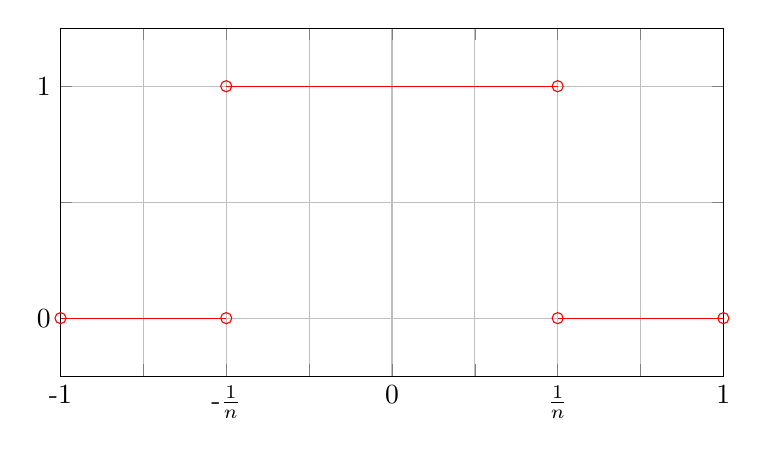
\begin{tikzpicture}
         \begin{axis}
        [width=10cm, height=6cm, xmin=-1, xmax=1, ymin=-0.25, ymax=1.25, xmajorgrids=true, ymajorgrids=true, xtick={-1,-0.75,-0.5,-0.25,0,0.25,0.5,0.75,1},  xticklabels={-1,,-$\frac{1}{n}$,,0,,$\frac{1}{n}$,,1}, ytick={0,0.5,1}, yticklabels={0,,1}]
        \addplot[color=red, mark=o] coordinates {(-1,0) (-0.5,0)};
        \addplot[color=red, mark=o] coordinates {(-0.5,1) (0.5,1)};
        \addplot[color=red, mark=o] coordinates {(0.5,0) (1,0)};
        \end{axis}
    \end{tikzpicture}
    \caption{Densidad uniforme $(-1/n$, $1/n)$.}
\end{figure}

Sea $f \in C_b(\R)$ una función continua y acotada, entonces la esperanza $\E(f(X_n))$ está dada por:
\[\E(f(X_n)) = \int_{\R}f(x)\mu_n(dx)\]
donde $\mu_n(dx)$ está dado por la densidad de la distribución de $X_n$, es decir la uniforme:\\ $$\mu_n(dx) = \frac{n}{2} \mathbbm{1}_{(-\frac{1}{n},\frac{1}{n})}(x)dx$$ 
Luego:
\[\E(f(X_n)) = \int_{\R}f(x)\,\frac{n}{2}\mathbbm{1}_{(-\frac{1}{n},\frac{1}{n})}(x)dx = \frac{n}{2}\int_{-\frac{1}{n}}^{\frac{1}{n}}f(x)dx\]

Haciendo uso del \textbf{teorema del valor medio} en integrales y de la continuidad de $f$, sabemos de la existencia de un valor $\xi_n \in (-\frac{1}{n},\frac{1}{n})$ tal que la integral anterior es de la forma:
\[\int_{-\frac{1}{n}}^{\frac{1}{n}}f(x)dx = \frac{2}{n}f(\xi_n)\]
Así,
\[\E(f(X_n)) = \frac{n}{2}\int_{-\frac{1}{n}}^{\frac{1}{n}}f(x)dx = f(\xi_n)\]
Por lo tanto la convergencia de $\E(f(X_n))$ estará dada por la convergencia de la nueva sucesión de puntos $(\xi_n)_{n\in\N}$. Para ver la convergencia de $\xi_n$ notemos que:
\begin{itemize}
    \item $\forall\,m\leq n$: $\left(-\frac{1}{n},\frac{1}{n}\right)\subset \left(-\frac{1}{m},\frac{1}{m}\right)$, por lo tanto:
    \[\xi_n \in \bigcap_{m=1}^{n}\left(-\frac{1}{m},\frac{1}{m}\right)\]
    Así la sucesión $\xi_n$ es acotada.
    \item Luego, la sucesión tiene al menos un punto de acumulación. Supongamos que $\Bar{\xi}$ es punto de acumulación de $(\xi_n)_n$, por lo dicho anteriormente debería suceder que:
    \[\Bar{\xi} \in \bigcap_{n\geq 1}\left(-\frac{1}{n},\frac{1}{n}\right) = \{0\}\]
    Finalmente se deduce que $\Bar{\xi}=0$.
\end{itemize}
Nuevamente, aplicando la continuidad de $f$:
\[\E(f(X_n)) = f(\xi_n) \rightarrow\,f(0) = \langle \delta_{0},f\rangle = \E(f(0))\]
\newline
Así concluimos que:
\begin{itemize}
    \item $\mu_n \Rightarrow\,\delta_{0}$, donde $\mu_n$ estaba dada por las distribuciones uniformes.
    \item $X_n \xrightarrow{\mathcal{L}}\,X$, donde $X\equiv 0$.
\end{itemize}
\textbf{Ejemplo 3:}
    Nuevamente tomamos como ejemplo $E=\R$, y definimos la siguiente medida:
    \[\mu_n = \frac{1}{n+1}\sum_{k=0}^{n}\delta_{k/n}\]
    
    De forma alternativa, definiendo $\mu_n = \mathcal{L}(X_n)$, donde $X_n$ corresponde al experimento de escoger un valor al azar del conjunto $\{0,\frac{1}{n},\frac{2}{n},\cdots,\frac{n}{n}\}$ y sea $\mu = \mathcal{L}(X)$, con $X\sim unif(0,1)$. Entonces $\forall$ $f\in C_b(\R)$:
    \[\langle \mu_n ,f\rangle = \frac{1}{n+1}\sum_{k=0}^{n} \langle \delta_{k/n},f\rangle = \frac{1}{n+1}\sum_{k=0}^{n}f(k/n)\]
    
    Notando que, para cada $n\in\N$ el conjunto $\{\frac{k}{n}\,|\,k=0,\cdots,n\}$ representa un refinamiento del intervalo $[0,1]$ y $f$ es una función acotada y contínua en ese intervalo (por lo tanto es \textit{Riemann-integrable}), entonces la suma anterior converge por ser suma de Riemann, y:
    \[\langle \mu_n ,f\rangle = \frac{1}{n+1}\sum_{k=0}^{n}f(k/n) \xrightarrow{n\rightarrow\infty}\, \int_{0}^{1}f(x)dx = \langle \mu,f\rangle\]
    Luego $\mu_n \Rightarrow\,\mu$, i.e. $X_n \xrightarrow{\mathcal{L}}\,X$.


\subsubsection{El Teorema Portmanteau}
\hspace{3.5mm}El siguiente teorema nos proporciona útiles equivalencias a la convergencia débil; cada una de ellas sirve como una definición. Un conjunto $A \in \mathcal{B}(E)$ cuya frontera $\partial A$ satisfaga que $\mu(\partial A) = 0$ se dirá conjunto \textit{$\mu$-contínuo} (Note que $\partial A$ es cerrado, por lo tanto pertenece a $\mathcal{B}(E)$).
\begin{teorema}[Portmanteau] Sean $\mu_n,\mu \in \mathcal{P}(E)$. Las siguientes proposiciones son equivalentes:
\begin{itemize}
    \item[i)] $\mu_n \Rightarrow \mu$
    \item[ii)] $\langle \mu_n,f\rangle \rightarrow\, \langle \mu, f\rangle$ para toda función $f$ acotada y uniformemente contínua.
    \item[iii)] $\langle \mu_n , f \rangle \rightarrow\, \langle \mu, f\rangle$ para toda función $f$, Lipschitz.
    \item[iv)] $\limsup_n \mu_n(F) \leq \mu(F)$   $\forall F \subset E$ cerrado.
    \item[v)] $\liminf_n \mu_n(G) \geq \mu(G)$     $\forall G\subset E$ abierto.
    \item[vi)] $\lim\, \mu_n(A) = \mu(A)$ para todo $A$, conjunto \textit{$\mu$-contínuo}. 
\end{itemize}
\end{teorema}

Notemos que, en el caso del \textbf{Ejemplo 1}, la desigualdad del punto $iii)$ se satisface estrictamente si $F=\{0\}$, de la misma forma en el punto $iv)$ si $G=\{0\}^{c}$. Si tomamos $A=\{0\}$, la convergencia no se alcanza en el punto $vi)$, pero esto no contradice el teorema, ya que la medida límite de $\partial \{0\} = \{0\}$ es 1, no 0. 
\\ \newline
\textbf{Demostración (Portmanteau):} Dado que las funciones uniformemente continuas, en particular son continuas, la implicancia $i)\rightarrow ii)$ se desprende trivialmente de la definición de convergencia débil en $i)$. Así mismo la implicancia $ii) \rightarrow iii)$ considerando las funciones Lipschitz.\\
Veamos la implicancia $iii) \rightarrow iv)$: \\ 

Sea $F$ un conjunto cerrado. $\forall \epsilon > 0$, sea:
\begin{equation}
   f(x) = \max\left(1-\frac{d(x,F)}{\epsilon}, 0\right)
   \label{eq:dem1}
\end{equation}

Donde $d(x,F)$ está dado por la métrica del espacio $E$. Se puede probar que la función $f$ definida de esta forma es $\frac{1}{\epsilon}$-Lipschitz y vale 1 en todo $F$. Además:
\begin{equation}
    \mathbbm{1}_F \leq f \leq \mathbbm{1}_{F^{\epsilon}}\hspace{1cm}\text{donde }F^{\epsilon}:=\{x\in E\,|\,d(x,F)<\epsilon\}\
    \label{eq:demostracionprtmanteau}
\end{equation}

Luego, integrando (bajo $\mu_n$) en las dos primeras partes de la desigualdad y aplicando límite superior:
\[\limsup\,\mu_n(F)\leq \limsup\,\langle \mu_n,f\rangle\]

Pero, como habíamos dicho, al ser $f$ una función Lipschitz, por la proposición $iii)$; $\langle \mu_n,f\rangle$ converge, por lo tanto el límite superior en realidad es el límite, más aún, converge en términos de $\mu$:
\begin{equation}
    \limsup \langle \mu_n,f\rangle = \lim \langle\mu_n,f\rangle = \langle \mu,f\rangle
\end{equation}

Ahora, nuevamente por la expresión en \ref{eq:demostracionprtmanteau}, integrando la segunda desigualdad (ahora bajo $\mu$):
\[\langle\mu,f\rangle \leq \mu(F^{\epsilon})\]

En resumen, tenemos que:
\[\limsup\,\mu_n(F) \leq \langle\mu,f\rangle \leq\mu(F^{\epsilon})\]

Al ser $F$ cerrado y $F^{\epsilon} \searrow F$, por continuidad de la medida se tiene que $\mu(F^{\epsilon})\searrow \mu(F)$ al momento que $\epsilon \rightarrow 0$ concluyendo el resultado.

\begin{figure}[H]
\centering
    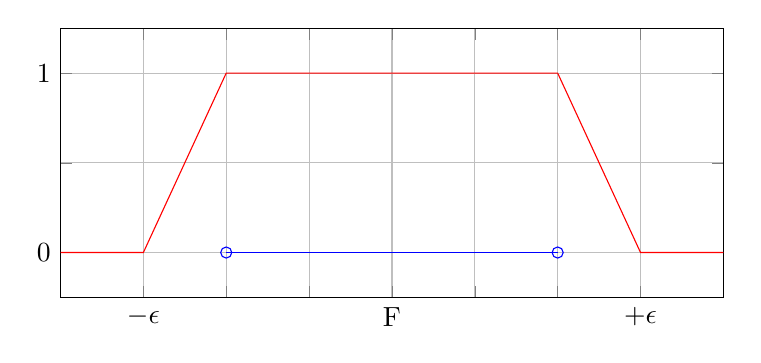
\begin{tikzpicture}
         \begin{axis}
        [width=10cm, height=5cm, xmin=-1, xmax=1, ymin=-0.25, ymax=1.25, xmajorgrids=true, ymajorgrids=true, xtick={-1,-0.75,-0.5,-0.25,0,0.25,0.5,0.75,1},  xticklabels={,$-\epsilon$,,,F,,,$+\epsilon$,}, ytick={0,0.5,1}, yticklabels={0,,1}]
        \addplot[color=red] coordinates {(-1,0) (-0.75,0) (-0.75,0) (-0.5,1) (-0.5,1) (0.5,1) (0.5,1) (0.75,0) (0.75,0) (1,0)};
        \addplot[color=blue, mark = o] coordinates {(-0.5,0) (0.5,0)};
        \end{axis}
    \end{tikzpicture}
    \caption{Esquema función f en \ref{eq:dem1}}
\end{figure}

Es directo ver que la proposición $iv)$ y $v)$ son equivalentes, así que la implicancia $iv) \rightarrow v)$ es directa de tomar complemento y utilizar que $\mu_n$ y $\mu$ son medidas de probabilidad.\\ 

Veamos que $iv)\land v)$ implican a $vi)$: Sea $A$ un conjunto $\mu$-contínuo. Dado que $\Bar{A}$ es cerrado, $A^{\circ}$ es abierto, ocupando la proposición $iv)$ y $A^{\circ} \subset A\subset \Bar{A}$:
\[\mu(\Bar{A}) \geq \limsup\,\mu_n(\Bar{A}) \geq \limsup\,\mu_n(A)\geq \liminf\,\mu_n(A) \geq \liminf\,\mu_n(A^{\circ})\geq \mu(A^{\circ})\]

Además, como $A$ es $\mu$-continuo: $\mu(\partial A) = 0$, entonces $\mu(\Bar{A}) = \mu(A^{\circ}) = \mu(A)$, por lo tanto todas las desigualdades anteriores son, en realidad, igualdades. Concluimos así que:
\begin{itemize}
    \item $\liminf\,\mu_n(A) = \limsup\,\mu_n(A)$ por lo tanto el límite existe.
    \item $\mu(A)\geq \lim\,\mu_n(A)\geq \mu(A)$, por lo tanto $\lim\,\mu_n(A) = \mu(A)$.
\end{itemize}

Por último, para finalizar, veremos la implicancia $vi)\rightarrow i)$:\\

Sea $f\in C_b(E)$, sin pérdida de generalidad podemos suponer que $0\leq f\leq 1$. En caso contrario, como $f$ es una función acotada, su supremo e ínfimo son finitos, por lo tanto podríamos definir una normalización para $f$:
\[\Tilde{f} = \frac{f - \inf_x f}{\sup_x f - \inf_x f}\]

Para la siguiente demostración haremos uso del siguiente resultado:
\begin{lem} Sea $g$ una función positiva, entonces:
    \begin{equation}
        \E_{\mu}(g(X)) = \langle\mu,g\rangle = \int_0^{\infty}\mu(g>t)dt
    \end{equation}
\end{lem}
\textbf{Demostración (Lema 1):} La primera igualdad es la definición de esperanza:
\[\E_{\mu}(g(X)) = \int_{0}^{\infty}g(x)\mu(dx)\]

Al mismo tiempo, podemos reescribir la función $g$ de la forma:
\[\E_{\mu}(g(X)) = \int_{0}^{\infty}\left(\int_{0}^{g(x)}dt\right)\,\mu(dx)\]

Ahora podemos extender la integral en $dt$ a todo el intervalo positivo mediante una indicatriz que anule los valores superiores a $g(x)$, esto es:
\[\E_{\mu}(g(X)) = \int_{0}^{\infty}\left(\int_{0}^{\infty}\mathbbm{1}_{\{g>t\}}dt\right)\mu(dx) = \int_{0}^{\infty}\int_{0}^{\infty}\mathbbm{1}_{\{g>t\}}dt\mu(dx)\]

Ocupando el teorema de Fubini podemos intercambiar el orden de las integrales, entonces:
\[\E_{\mu}(g(X)) = \int_{0}^{\infty}\int_{0}^{\infty}\mathbbm{1}_{\{g>t\}}dt\mu(dx) = \int_{0}^{\infty}\int_{0}^{\infty}\mathbbm{1}_{\{g>t\}}\mu(dx)dt = \int_{0}^{\infty}\mu(g>t)dt\]
\rule{0.7em}{0.7em}

Entonces, volviendo a la demostración del teorema, tenemos que:
\[\langle \mu,f\rangle = \int_{0}^{1}\mu(f>t)dt\]
\[\langle \mu_n , f \rangle = \int_{0}^{1}\mu_n(f>t)dt\]

Donde el intervalo de integración lo podemos acotar, puesto que definimos el rango de la función $f$ en $[0,1]$. Además, como $f$ es contínua, es fácil ver que:
\[\partial \{f>t\} \subset\,\{f=t\}\]

Notemos que $\mu(f=t)=0$ salvo para, a lo más numerables, valores de t's. De lo contrario, la medida $\mu$ no sería finita. Luego, $dt-c.s.$ tenemos:
\[\mu(\partial\{f>t\}) \leq \mu(\{f=t\}) = 0\]

Es decir: de manera $dt-c.s.$ $\{f>t\}$ es $\mu$-contínuo. Por la proposición $vi)$:
\[\mu_n(f>t) \xrightarrow{\,\,n\,\,}\,\mu(f>t)\hspace{1cm}dt-c.s.\]

Finalmente, ocupando el \textbf{T.C.D.}:
\[\langle\mu_n,f\rangle = \int_{0}^{\infty}\mu_n(f>t)dt \xrightarrow{\,\,\,\textbf{T.C.D.}\,\,\,}\int_{0}^{\infty}\mu(f>t)dt = \langle \mu,f\rangle\]
\rule{0.7em}{0.7em}

Habiendo establecido anteriormente, la equivalencia entre la convergencia débil de medidas de probabilidad y la convergencia en LEY de variables aleatorias, podemos enunciar el Teorema Portmanteau para variables aleatorias.

\begin{teorema}[Portmanteau para variables aleatorias.] Sean $(X_n)_{n\in\N}$, $X$ variables aleatorias en $(E,d)$ espacio métrico. Las siguientes proposiciones son equivalentes:
\begin{enumerate}
    \item[i)] $X_n\,\xrightarrow{\mathcal{L}}\,X$
    \item[ii)] $\E(f(X_n)) \xrightarrow{\,\,n\,\,}\E(f(X))$ para toda función $f$ acotada y uniformemente continua.
    \item[iii)] $\E(f(X_n)) \xrightarrow{\,\,n\,\,}\E(f(X))$ para toda función $f$ Lipschitz.
    \item[iv)] $\limsup\,\pb(X_n \in F) \leq \pb(X\in F)$ $\forall F\subset E$ cerrado.
    \item[v)] $\liminf\,\pb(X_n \in G) \geq \pb(X \in G)$ $\forall G\subset E$ abierto.
    \item[vi)] $\lim \pb(X_n \in A) = \pb(X\in A)$ para todo $A\in \mathcal{B}(E)$ conjunto $\mu$-continuo ( $\pb(X \in \partial A) = 0$ ).
\end{enumerate}
\end{teorema}

\textbf{Observación 1:} Tomando $E=\R$, la condición $vi)$ del teorema suele ser interesante, como en el siguiente ejemplo:\\

Sabemos de ejemplos anteriores que:
\[\delta_{1/n}\Rightarrow \,\delta_{0}\]

Sin embargo, para el conjunto $A=(0,\infty)$, $\forall\,n\in\N$:
\[\delta_{1/n}(A) = 1\]
\[\delta_{0}(A) = 0\]

Es decir que $\delta_{1/n}(A)$ no converge a $\delta_{0}(A)$, sin embargo esto no contradice la condición $vi)$, pues el conjunto $A$ no es $\delta_0$-contínuo.
\[\delta_{0}(\partial A) = \delta_{0}(\{0\}) = 1\]


\subsubsection{El Teorema del Mapeo.}
\hspace{3.5mm}Supongamos que $h$ es una función de $(E,d)$ a otro espacio métrico, $(\hat{E},\hat{d})$. \\Si $h$ es $\mathcal{B}(E)/\mathcal{B}(\hat{E})$-medible, entonces cada medida de probabilidad $\mu \in \mathcal{P}(E)$ induce a otra medida de probabilidad $\mu h^{-1} \in \mathcal{P}(\hat{E})$, definida de la manera usual, como $\mu h^{-1}(A) = \mu(h^{-1}(A))$. \\

Necesitamos, entonces, condiciones bajo las cuales el hecho de tener una convergencia débil, $\mu_n \Rightarrow \mu$, en $\mathcal{P}(E)$, me implique una convergencia débil, $\mu_nh^{-1} \Rightarrow \mu h^{-1}$ para medidas en $\mathcal{P}(\hat{E})$. \\ 

Una de las condiciones pensadas para $h$ podrías ser la continuidad, pero veremos que esta condición puede ser reemplazada por una más débil. Asumimos que $h$ será una función $\mathcal{B}(E)/\mathcal{B}(\hat{E})$-medible, y sea $D_h$ el conjunto de los puntos de discontinuidad de la función $h$ ($D_h \in \mathcal{B}(E)$). Tenemos el siguiente resultado;  si $\mu_n \Rightarrow\,\mu$ y $\mu(D_h) = 0$, entonces $\mu_n h^{-1} \Rightarrow\, \mu h^{-1}$. \\

En otras palabras:

\begin{teorema}[Del Mapeo.] Sea $(\hat{E},\hat{d})$ otro espacio métrico y sea $h:\,E\rightarrow\,\hat{E}$, una función medible. $(X_n)_{n\in\N}$, $X$ son variables aleatorias en $E$.\\ \newline
Si $X_n\,\xrightarrow{\mathcal{L}}\,X$ y $\pb(X \in D_h) = 0$, entonces: $h(X_n) \,\xrightarrow{\mathcal{L}}\,h(X)$. Donde $D_h :=\{x\in E\,|\,\text{$h$ es discontínua en x}\}$
\end{teorema}
\textbf{Demostración:} Sea $B \subset\,\hat{E}$, un conjunto $\mathcal{L}(h(X))$-continua, es decir:
\begin{equation}
    \pb(h(X) \in \partial B) = 0
    \label{eq:dem2}
\end{equation}

Por el teorema Portmanteau en variables aleatorias, la convergencia en LEY es equivalente a decir que:
\[\pb(h(X_n)\in B) \xrightarrow{\,\,n\,\,}\,\pb(h(X)\in B)\]

Lo que a su vez, es equivalente a decir que:
\[\pb(X_n \in h^{-1}(B)) \xrightarrow{\,\,n\,\,}\,\pb(X \in h^{-1}(B))\]

Luego, basta con demostrar que $h^{-1}(B)$ es un conjunto $\mathcal{L}(X)$-contínuo, $i.e.$; falta por demostrar que $\pb(X \in \partial h^{-1}(B)) =0$.\\

Sea $x \not\in D_h$, luego:
\[\text{si }x\in\overline{h^{-1}(B)}\,\Rightarrow\,\exists\,x_n \in h^{-1}(B)\,\text{tal que }x_n\,\rightarrow\,x\]
\[\Rightarrow\,h(x)\in\,\overline{B}\]

Similarmente, si $x\not\in\,D_h$,
\[\text{si }x\in\,int\left(h^{-1}(B)\right)^{c}\,\Rightarrow\,\exists\,x_n \rightarrow\,x\,\text{ tal que  }x_n\,\not\in\,h^{-1}(B)\]
\[i.e:\hspace{0.2cm}h(x_n)\not\in\,B^{\circ}\]

Luego, para $x\not\in D_h$:
\[x\,\in\,\partial h^{-1}(B) \,\Rightarrow\,h(x)\in\partial B\,\hspace{1cm}\text{Es decir:}\]
\[\partial h^{-1}(B) \cap D_h^{c}\,\,\subset\,h^{-1}(\partial B)\cap D_h^{c}\,\,\subset\,h^{-1}(\partial B)\]

Así, y dado el hecho de que $D_h^{c}$ es un conjunto de medida $1$:
\[\pb(X \in \partial h^{-1}(B)) = \pb(X \in \partial h^{-1}(B) \cap D_h^{c}) \leq \pb(X \in h^{-1}(\partial B))=0\]

De donde la última igualdad se tiene por la hipótesis $\ref{eq:dem2}$.
\rule{0.7em}{0.7em}\\\newline
\textbf{Observación 1:} La convergencia en ley de $X_n$ a $X$ no requiere que los $X_n$ y $X$ estén definidos en el mismo espacio de probabilidades, puesto que para cada $n\in\N$ el espacio $(\Omega,\mathcal{F},\mu_n)$ va cambiando de medida, a diferencia de la convergencia $c.s.$ o en probabilidad.

\begin{prop}
Sean $(X_n)_{n\in\N}$ y $X$ variables aleatorias definidas sobre el mismo espacio de probabilidades. Entonces:
\[X_n\xrightarrow{\,\,c.s.\,\,} X \Rightarrow\,X_n \xrightarrow{\,\,\pb\,\,}X \Rightarrow\,X_n\,\xrightarrow{\,\,\mathcal{L}\,\,}X\]
\end{prop}
\textbf{Demostración: propuesto.}

\subsection{Tensión (Tightness)}
\subsubsection{Relativamente compacto.}
\hspace{3.5mm}Sea $M\subset \mathcal{P}(E)$ una familia de medidas de probabilidad sobre el espacio métrico $(E,d)$. Diremos que $M$ es \textbf{relativamente compacto} si cada sucesión de elementos en $M$ contiene una subsucesión que converge débilmente, es decir; si $\{\mu_n\}$ es una secuencia de elementos en $M$, entonces existe una subsucesión $\{\mu_{n_i}\}$ y una medida de probabilidad $\mu \in \mathcal{P}(E)$, tal que $\mu_{n_i} \Rightarrow \mu$.  \\ 

Notamos que esta caracterización evita la descripción topológica que se encuentra subyacente en las definiciones de \textit{compacidad} o \textit{convergencia}. Se puede mostrar la existencia de una métrica que dota al espacio de tal topología pero no es de vital importancia para este curso, he ahí el motivo de su ausencia en estas notas. \\

Sin embargo, notamos que esta definición genera cierto problema para probar que un conjunto de medidas es relativamente compacto, dada la escasa gama de herramientas que poseemos en este momento. Es por esto, que se introduce la siguiente definición:

\begin{definicion}[Tensión] Una familia $M\subseteq \mathcal{P}(E)$ se dice \textbf{TENSA} si $\forall \epsilon > 0$, $\exists K\subseteq E$ compacto tal que:
\[\mu(K) > 1-\epsilon \hspace{1cm}\forall\,\mu\in M\]
\end{definicion}
% \\ \newline

El siguiente resultado importante justifica la definición anterior:


\begin{teorema}[de Prohorov] Sea $M\subseteq \mathcal{P}(E)$.
\begin{itemize}
    \item[i)] Si $M$ es tensa, entonces es relativamente compacta.
    \item[ii)] Supongamos que $E$ es un espacio \textbf{polaco} (espacio métrico completo y separable). Si $M$ es relativamente compacta, entonces es tensa.
\end{itemize}
\end{teorema}

\begin{cor} Si $\{\mu_n\}$ es tensa y cada subsucesión débilmente convergente, converge a la misma medida $\mu\in\mathcal{P}(E)$, entonces toda la secuencia $\mu_n$ converge débilmente a $\mu$: $\mu_n \Rightarrow \mu$.
\end{cor}
\textbf{Demostración:} Ver \cite[págs. 59,69]{Bill}\\\newline
\textbf{Ejemplo 4:}
\begin{itemize}
    \item Si $E$ es compacto, entonces toda familia $M\subseteq \mathcal{P}(E)$ es tensa.
    \item En $E=\R$, sea $M=\{\delta_n \}$ el conjunto de las delta de Dirac en los puntos $n\in\N$. Claramente $M$ no es tensión, cada vez que proponemos un conjunto compacto, al ser la sucesión \\$\{n\,|\, n\in\N\}$ no acotada, existirá un $n$ suficientemente grande que se escape del compacto en $\R$. 
    \item En $E=\R$, sea $M=\{\mathcal{N}(0,n)\}_{n\in\N}$. $M$ no es tensión.
\begin{figure}[H]
\centering
    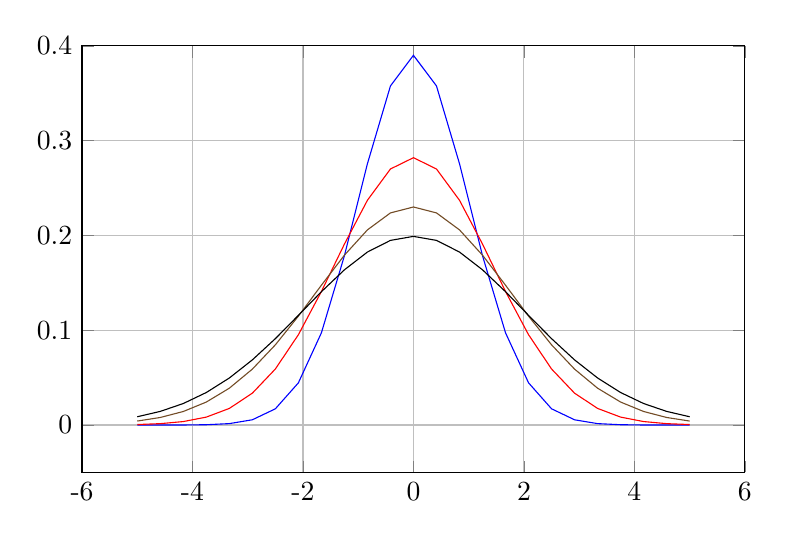
\begin{tikzpicture}
         \begin{axis}
        [width=10cm, height=7cm, xmin=-6, xmax=6, ymin=-0.05, ymax=0.4, xmajorgrids=true, ymajorgrids=true, xtick={-6,-4,-2,0,2,4,6},  xticklabels={-6,-4,-2,0,2,4,6}, ytick={0,0.1,0.2,0.3,0.4}, yticklabels={0,0.1,0.2,0.3,0.4}]
        
        \addplot+[no marks]{0.39*e^(-0.5*x^2)};
        \addplot+[no marks]{0.282*e^(-0.25*x^2)};
        \addplot+[no marks]{0.23*e^(-0.16*x^2)};
        \addplot+[no marks]{0.199*e^(-0.125*x^2)};
        \end{axis}
    \end{tikzpicture}
    \caption{Sucesión de densidades $\mathcal{N}(0,n)$.}
\end{figure}

    \item Sin embargo, considerando $E=\overline{\R}:=\R\cup \{-\infty ,+\infty\}$, entonces la sucesión $M=\{\delta_n \}_n$ es tensa pues: $\delta_n \Rightarrow \delta_{+\infty}$.
    
    \item De la misma forma, si $E=\overline{\R}$, la familia de medidas $M=\{\mathcal{N}(0,n)\}_n$, entonces:
    \[\mathcal{N}(0,n) \Rightarrow\,\frac{1}{2}\,\delta_{-\infty} + \frac{1}{2}\,\delta_{+\infty}\]
\end{itemize}
